\section{Evaluation}
We now evaluate the performance of Genesis along various dimensions:
 (1) What is the performance of Genesis in synthesizing simple reachability and waypoint policies
  with increasing number of policies and greater sizes of topologies and benchmarking the constraints used by the synthesis algorithm? 
  (2) How quickly can Genesis synthesize isolation policies in datacenter topologies for varying number of policies and percentage of
   datacenter utilization? 
   (3) What is the performance of Genesis for solving link-capacity policies in internet topologies? 
   (4) Identifying the benefits of tactics in terms of reduction of terms in the synthesis algorithm and actual benefits 
   with respect to synthesis without tactics for different isolation workloads in datacenter topologies? 
   (5) What are the potential speedups of using optimistic synthesis in Genesis for varying workloads? 

\begin{figure*}[width=2\columnwidth]
	\centering
	\subfloat[No Tactic]{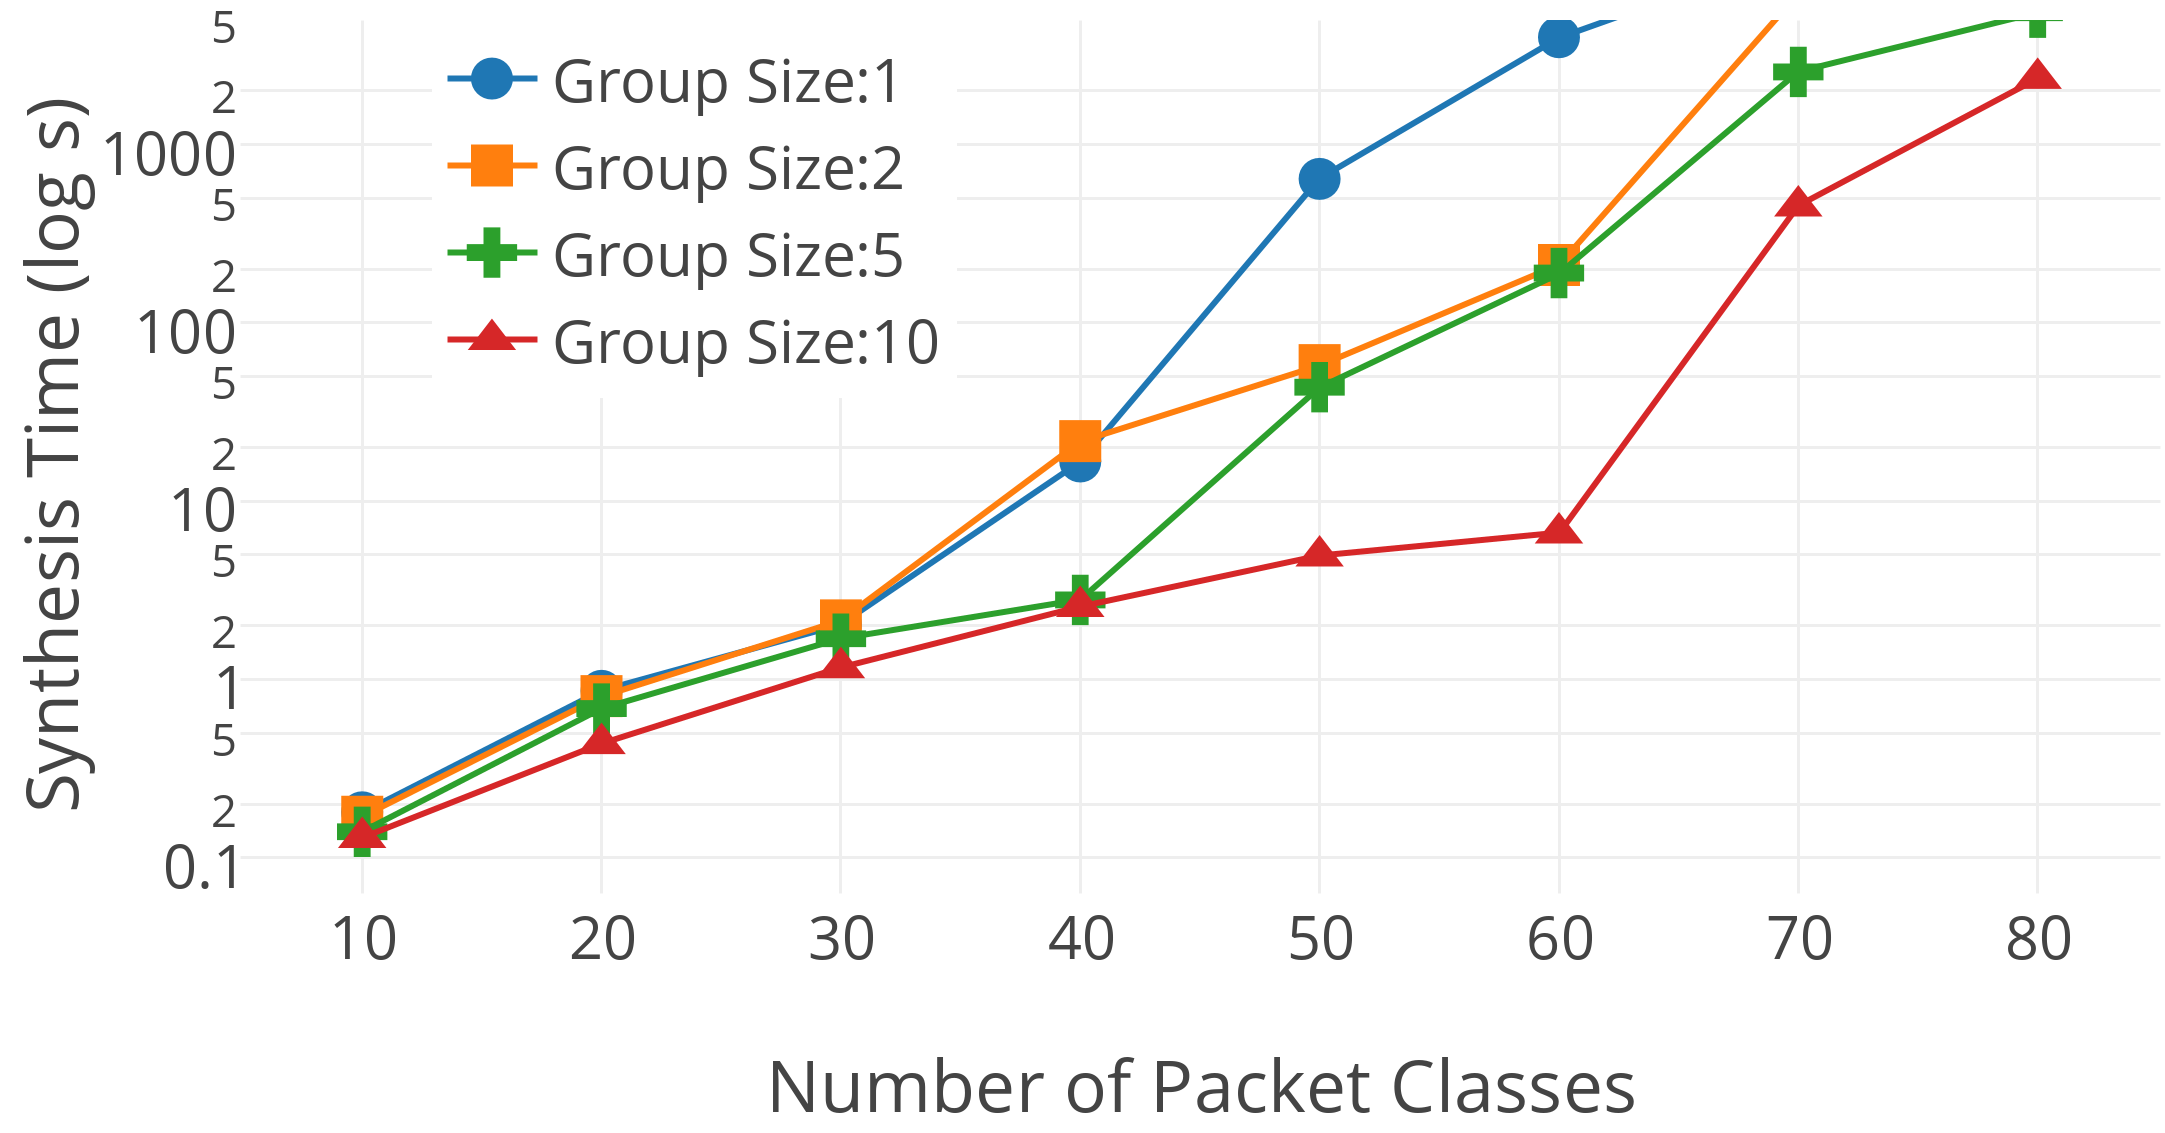
\includegraphics[width=0.66\columnwidth]{figures/no-tactic-isolation-plot.png}}
	\subfloat[No Edge Tactic]{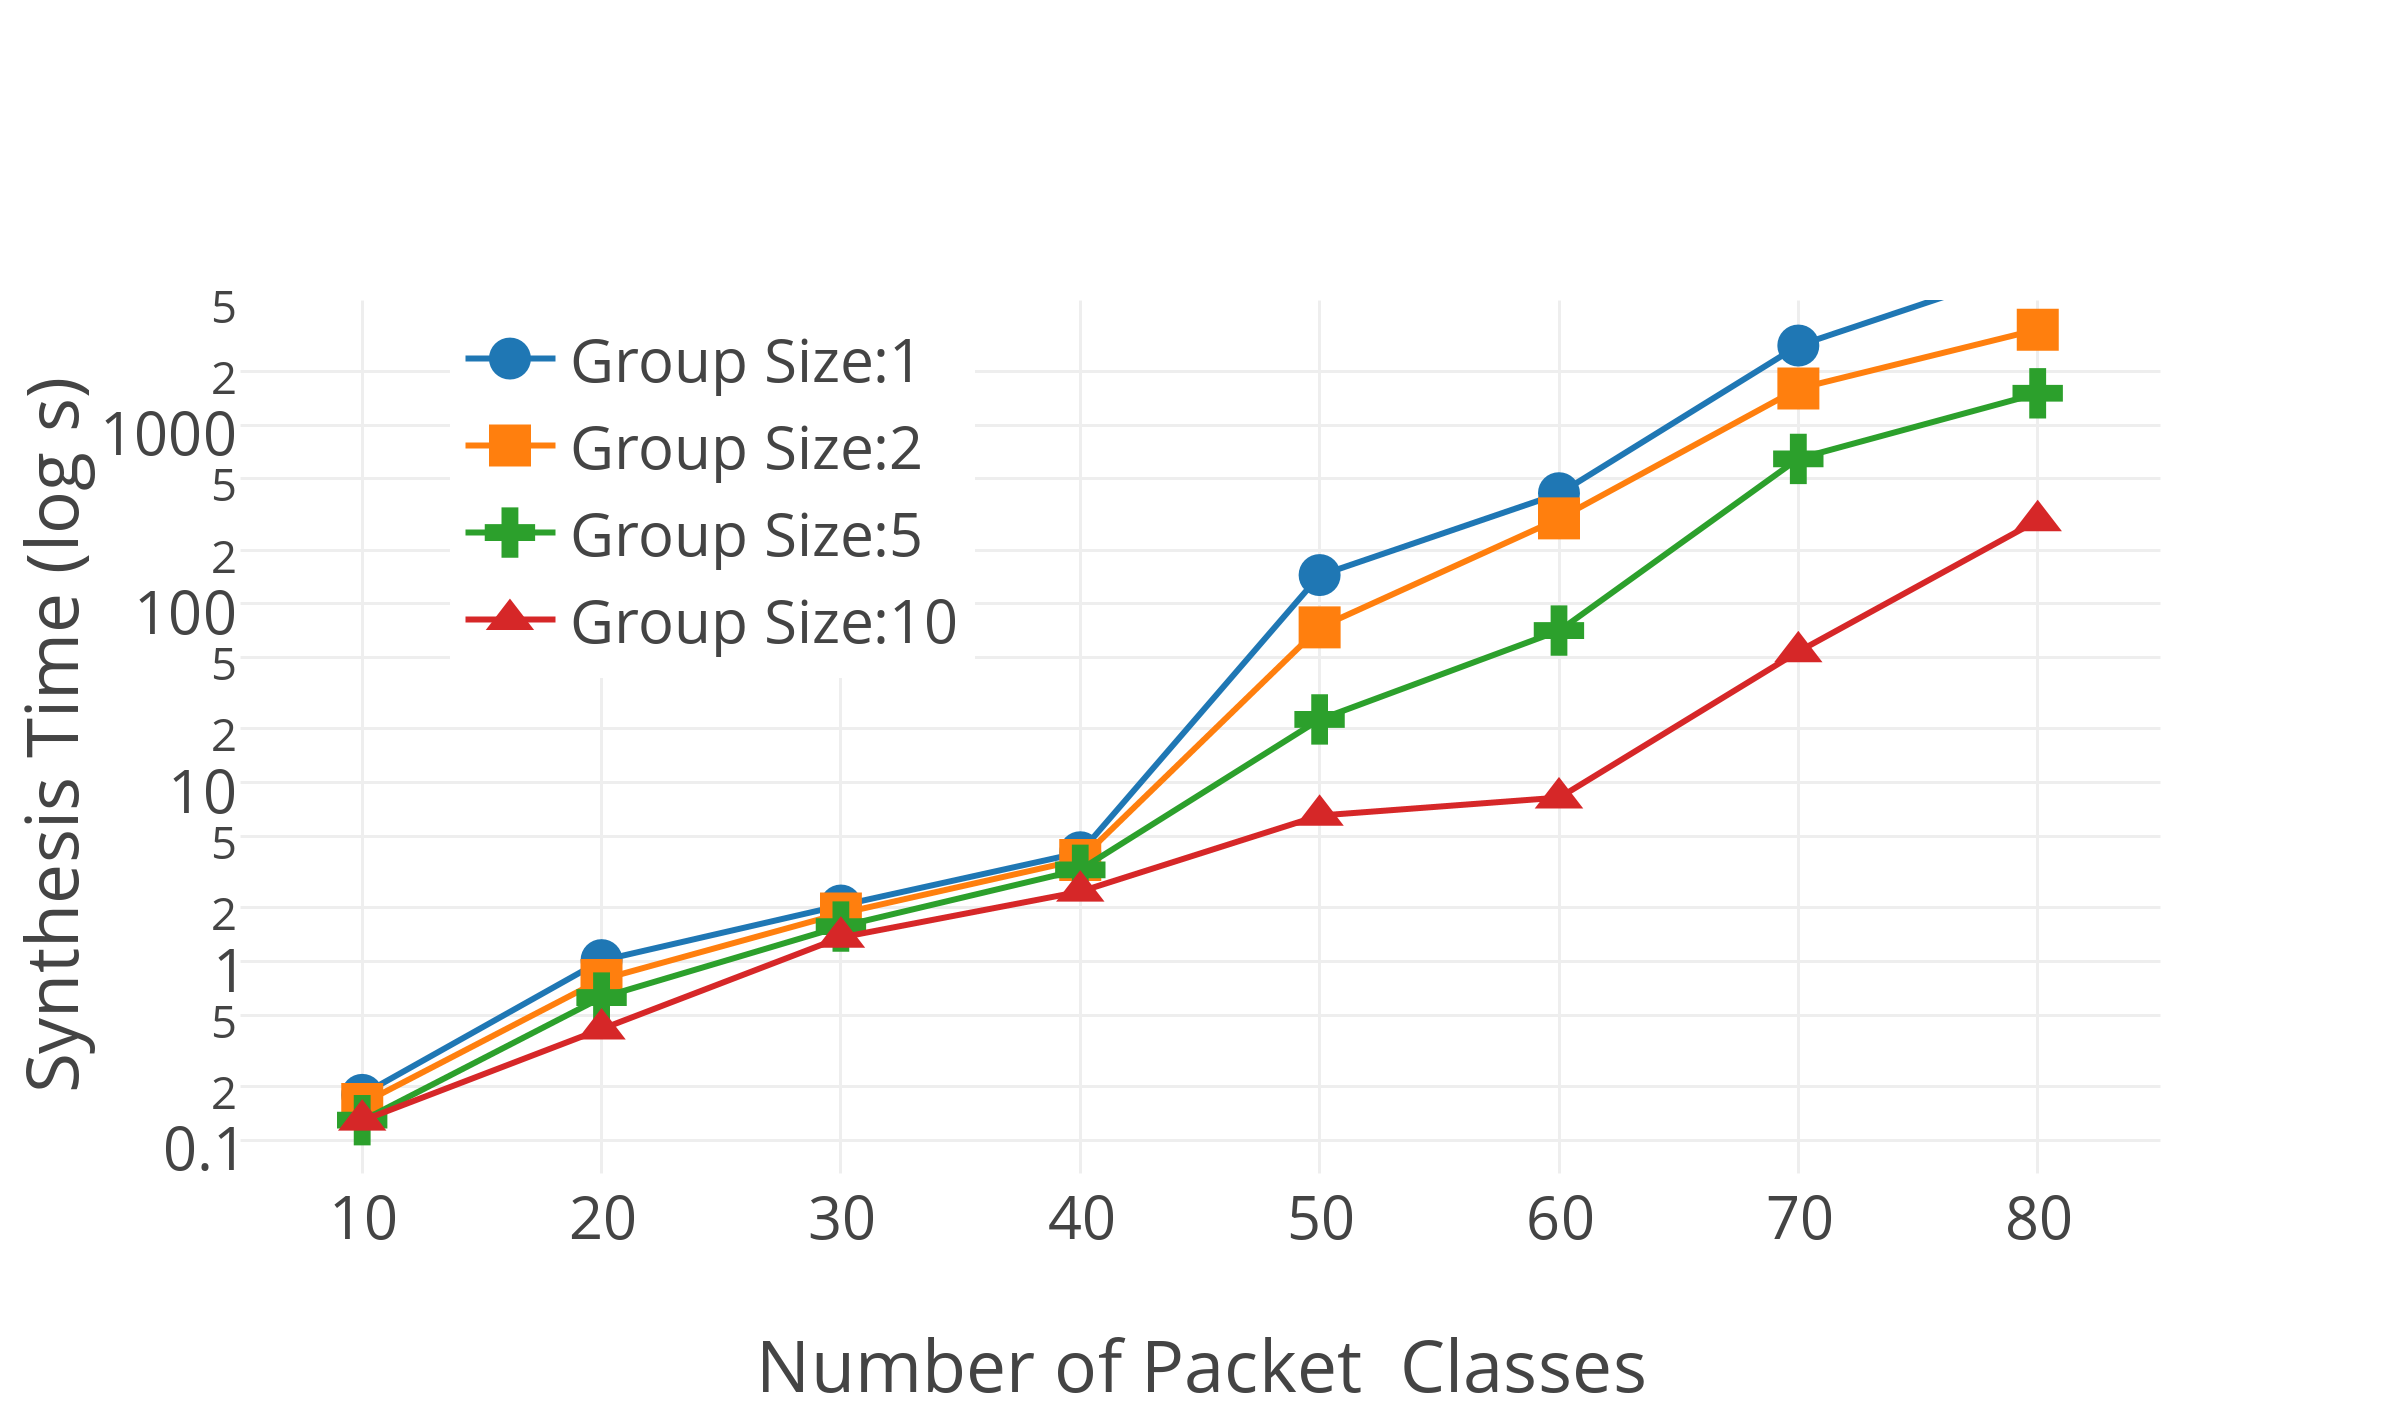
\includegraphics[width=0.66\columnwidth]{figures/no-edge-tactic-isolation-plot.png}}
	\subfloat[Valley-free Routing Tactic]{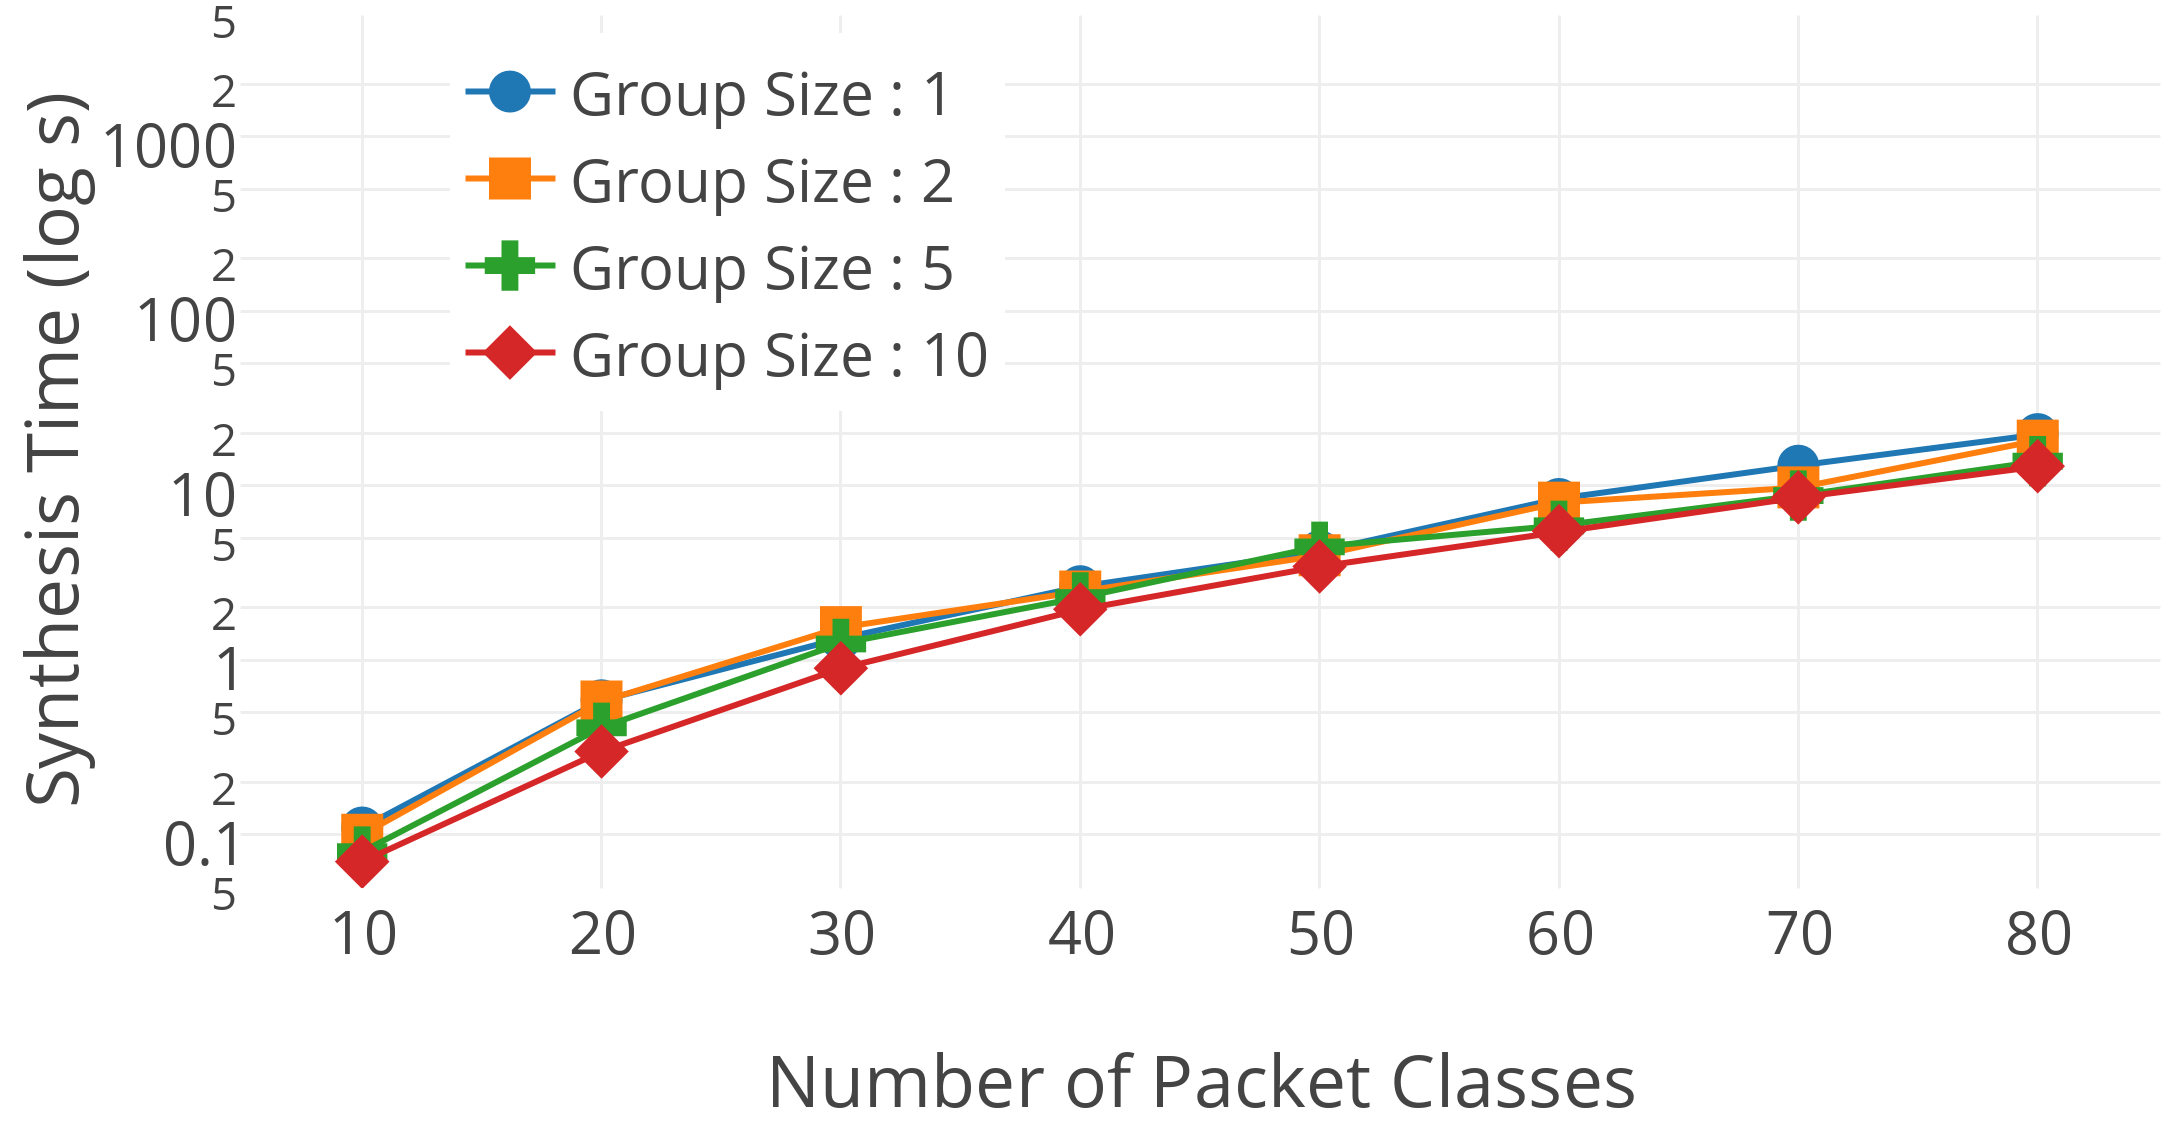
\includegraphics[width=0.66\columnwidth]{figures/eacae-isolation-plot.png}}
	\caption{\label{fig:tactic-isolation}
		Synthesis time (log scale) for isolation workloads over range of packet classes and different tenant-group sizes.}
\end{figure*}
\kausik{Needs another pass.}
We model our experimentation on a multi-tenant datacenter setting. We 
define a tenant-group flows as the reachability policies specified by a tenant
for its virtual machines. The primary metric we consider to evaluate \Name's 
performance is the time taken for the Z3 solver to find a solution after 
the system has added constraints for the policies for different workloads. \kausik{Footnote needed to ignore other times.}
We focus on synthesis of tenant-isolation
workloads for varying sizes of a fat-tree 
topology as a representative datacenter network. For tenant isolation, there are
no isolation policies with packet classes in a tenant-group, but each packet class
has a isolation policy with all other tenant-group packet classes. This setup ensures
that flows of a tenant can share links, but flows of two different tenants cannot share
any link. 
For empirical purposes, 
we randomly
\footnote{Smarter placement of tenants could speed-up synthesis as tenant endpoints would
	be located closer to each other. The placement algorithm can be used to develop specialised tactics.}
  pack the tenant's virtual machines on racks connected to edge switches such that
   we do not place virtual machines of different tenants on the same rack which would 
   cause isolation to fail at the edge switch itself (due to bounded number of links at
   the edge switch). Operators can aggregate a tenant's traffic from one rack to
another to a single reachability policy and find pathways for communication amongst the multiple
machines in different racks. 
All experiments were conducted using a Cloudlab machine with 32-core Intel-Xeon 2.40GHz CPU and 128Gb of RAM. 
\subsection{Isolation Workloads}
The synthesis time (we cap the maximum time at 5000s) for a range of
 packet classes with varying tenant-group sizes in 80 node fat-tree topology (pod size = 8) 
 without tactics is shown in \cref{fig:no-tactic}. For example, the total packet classes is 50, and group size is 5 means there
  are $50/5 = 10$ tenants, and each tenant flow in the group is isolated with all other tenant
   flows. For a fixed group size, we can observe that as number of packet classes increases,
    the synthesis time increases expotentially, as expected. As we decrease group size,
     we can observe that synthesis time increases greatly for the same number of policies,
      as the number of tenants increases, consequently the problem is more constrainted 
      due to increased number of isolation policies. 
      Group size = 1 denotes the extreme case where all flows are isolated to one other. 
      
%\begin{figure}[H]
%	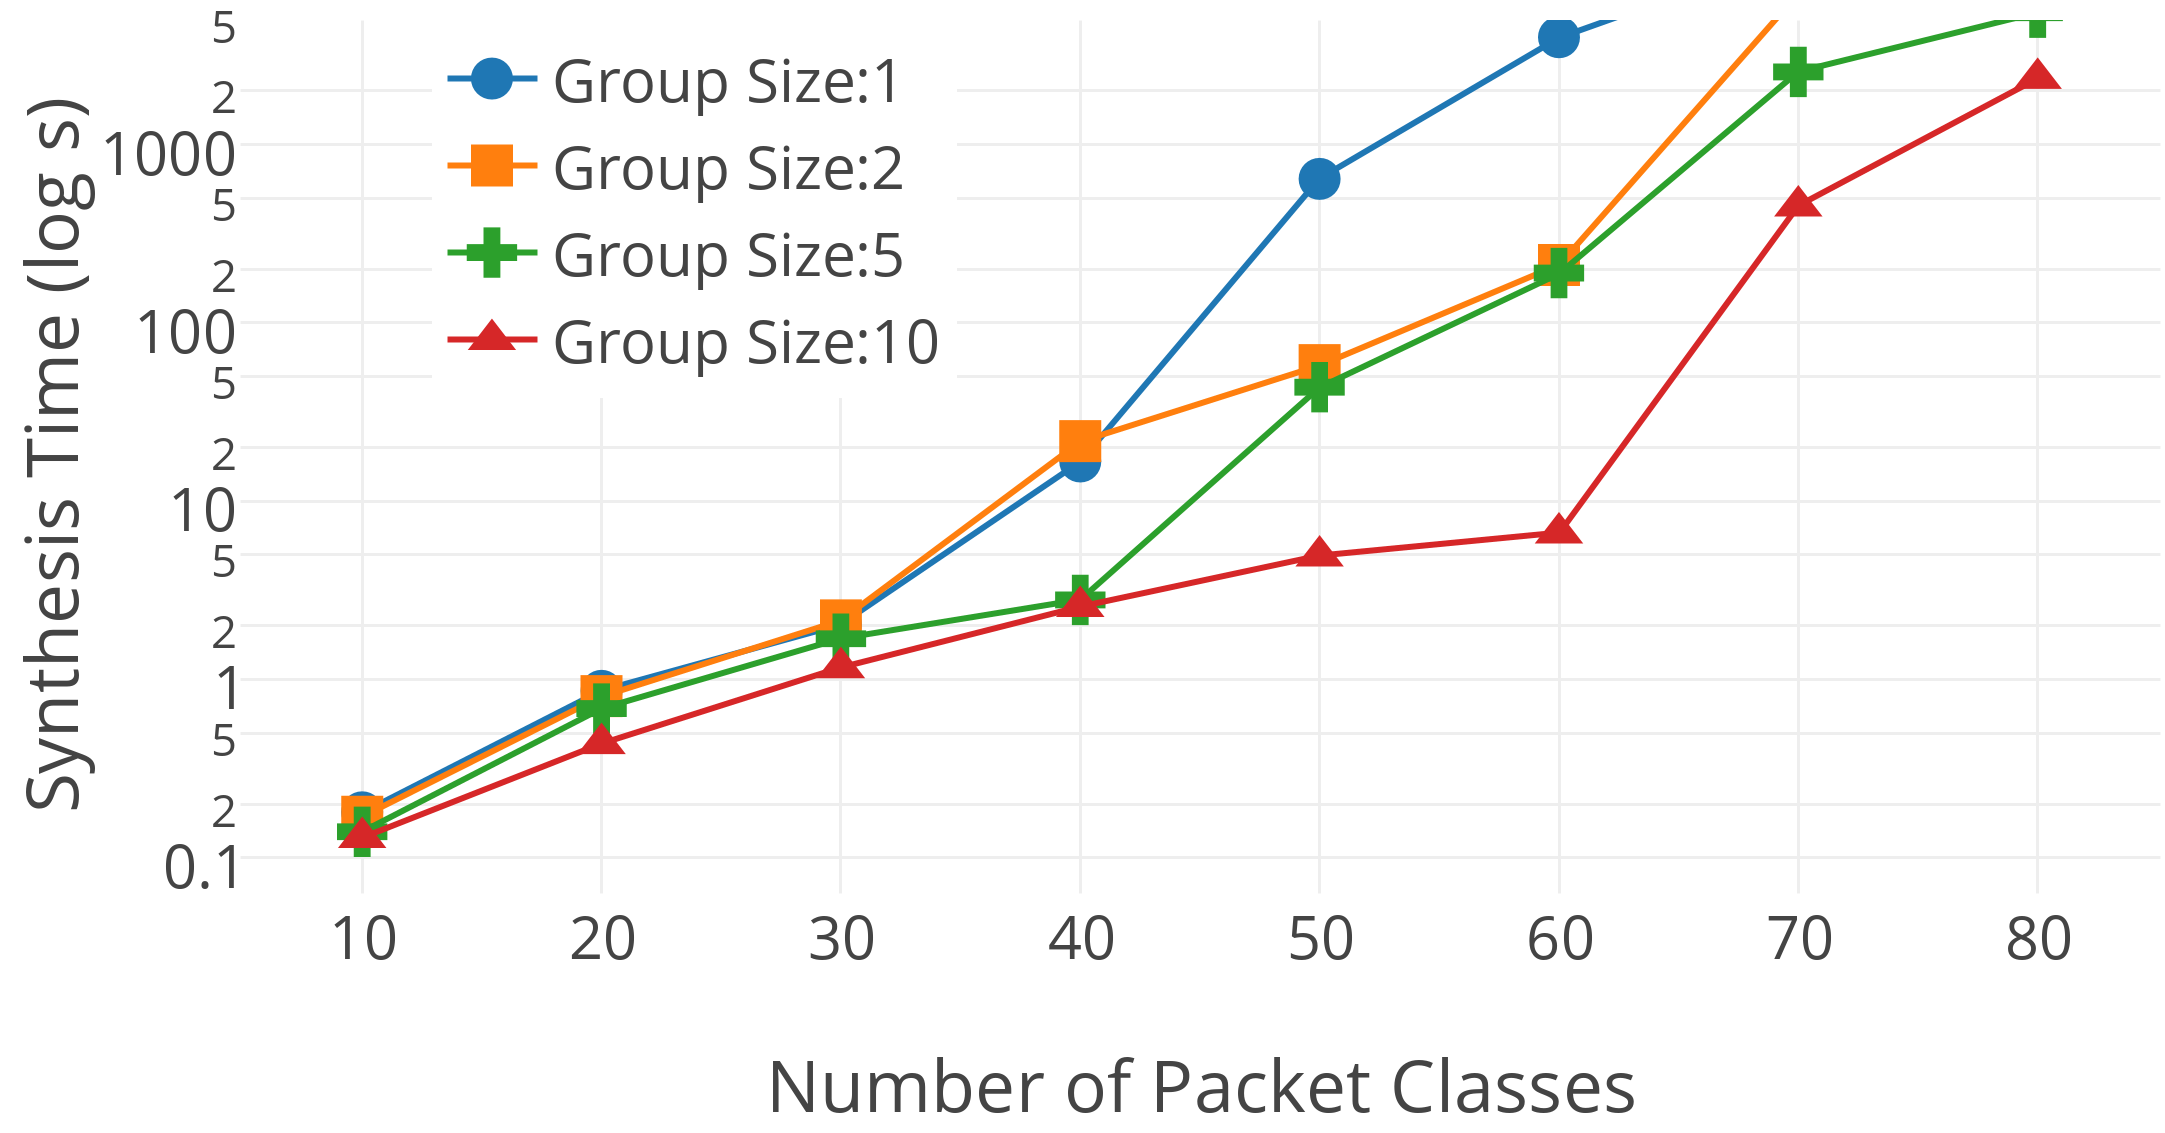
\includegraphics[width=\columnwidth]{figures/no-tactic-isolation-plot.png}
%	\caption{Synthesis time (log scale) with no tactics for range of packet classes and different tenant-group sizes.}
%	\label{fig:no-tactic}
%\end{figure}

\begin{figure}[H]
		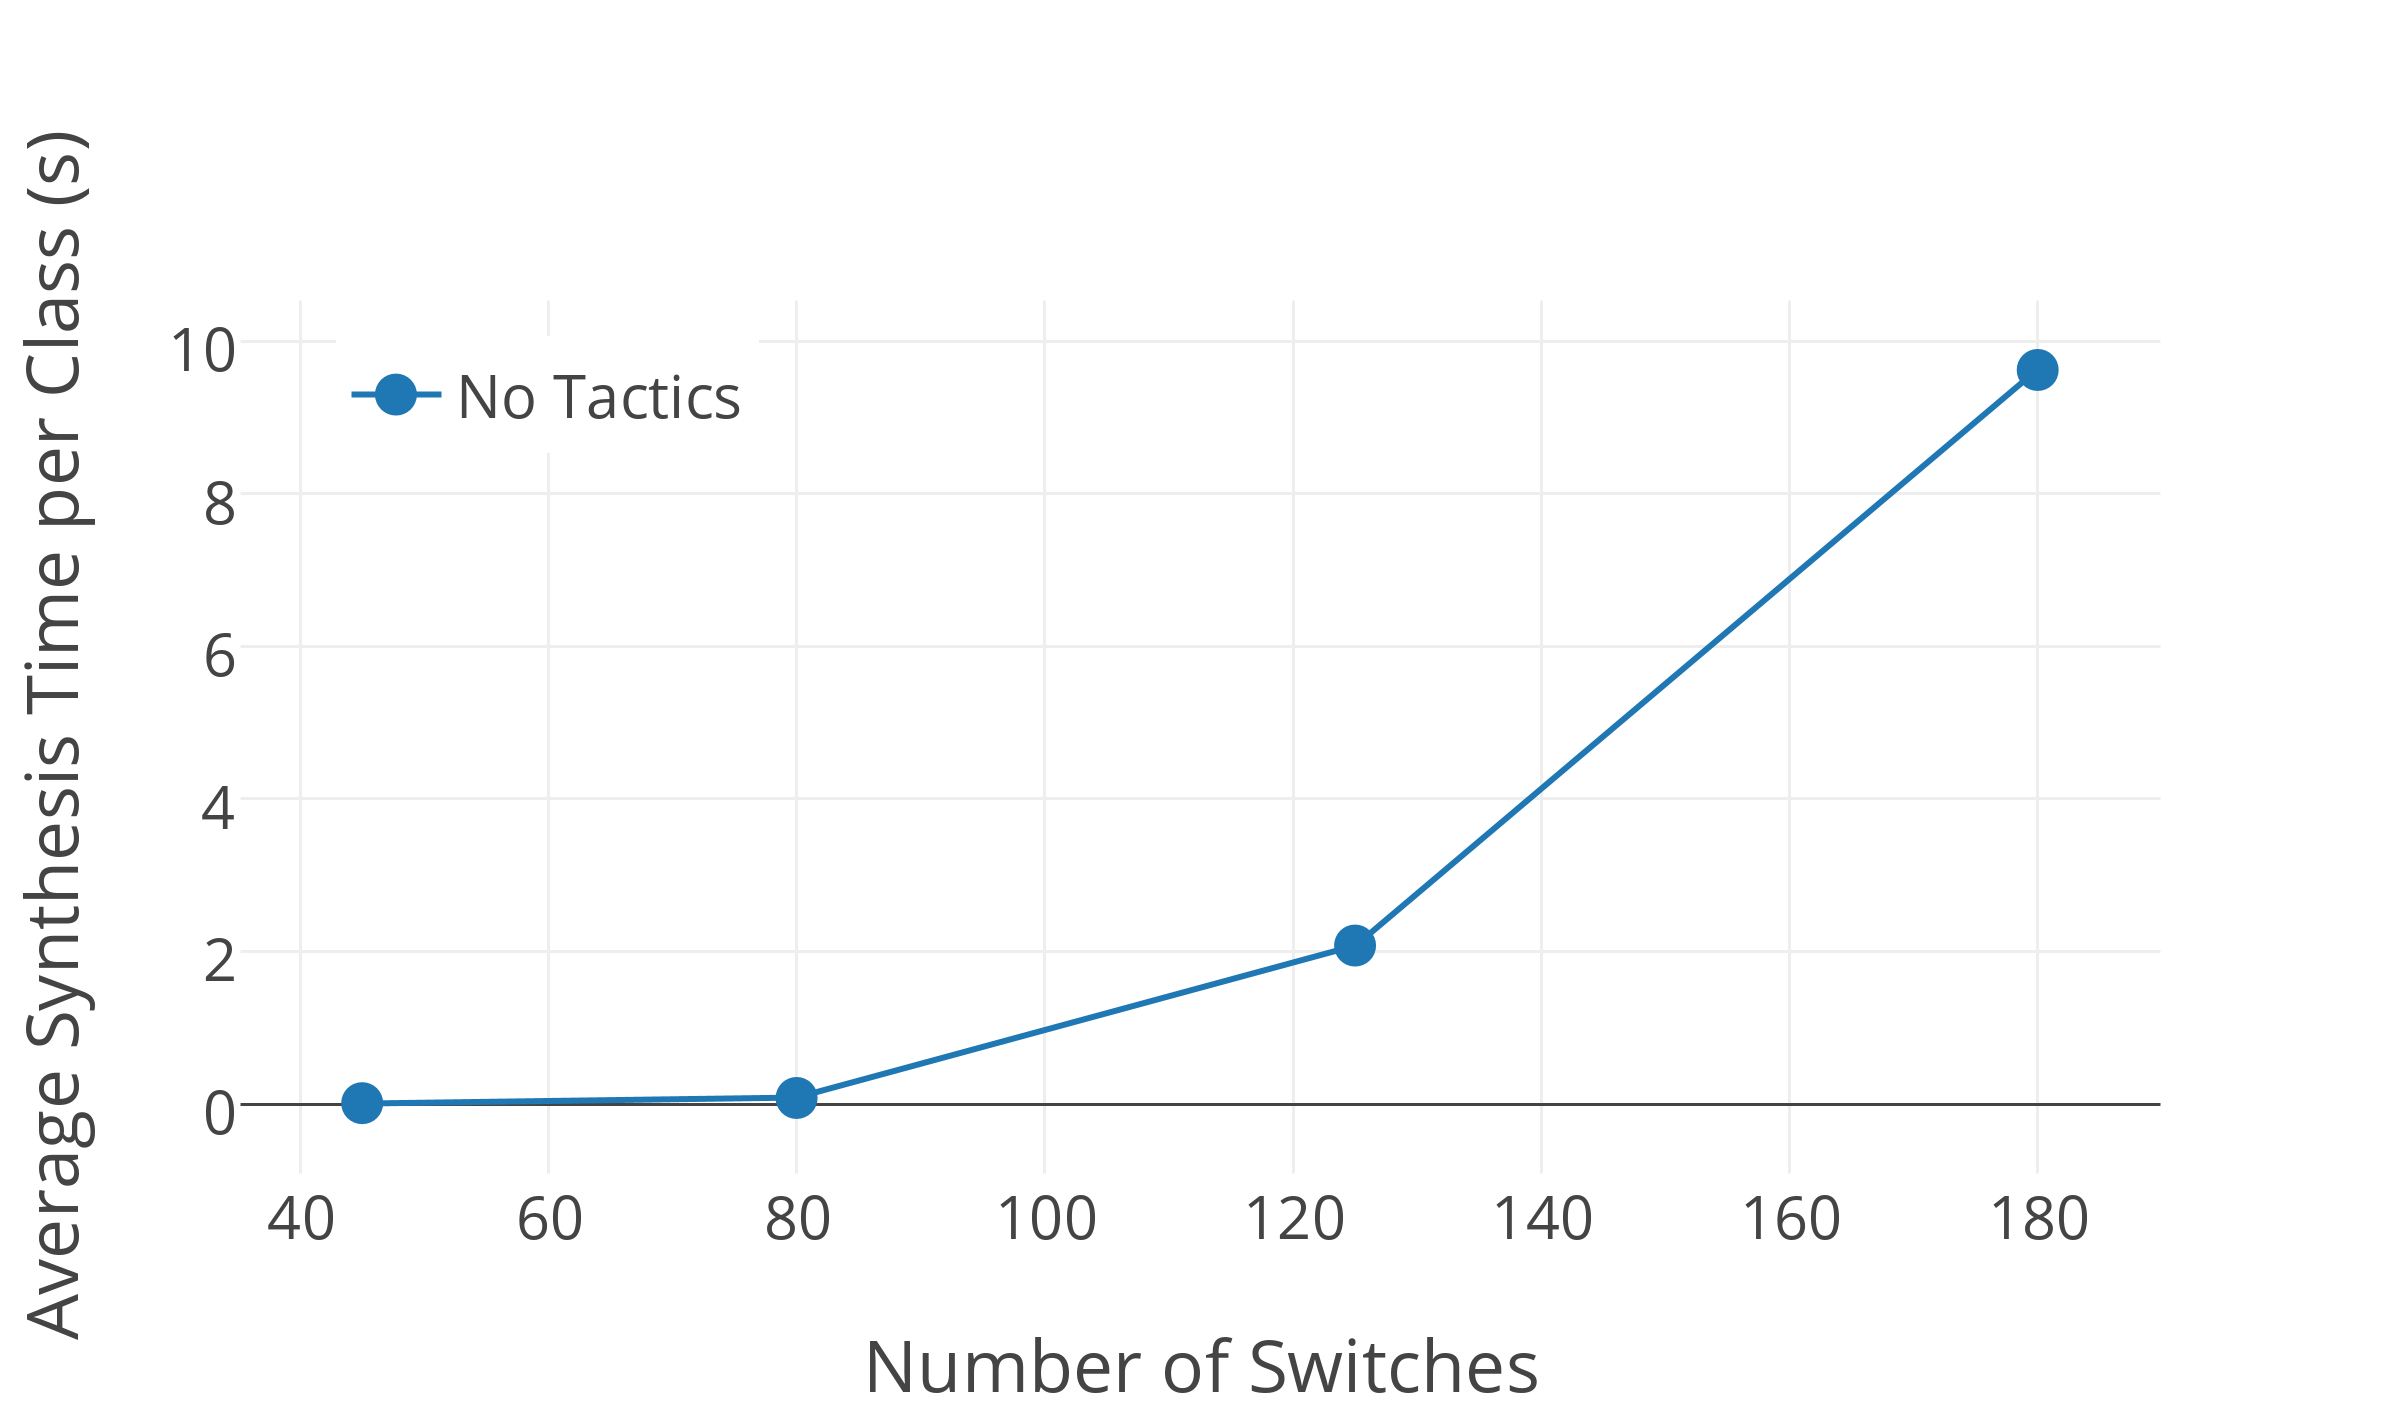
\includegraphics[width=\columnwidth]{figures/no-tactic-topo.png}
		\caption{Average synthesis time per packet class versus fat-tree topology size for isolation workloads with datacenter packing ratio 0.25.}
		\label{fig:no-tactic-topo}
\end{figure}


The average synthesis time per class for isolation workloads
 on increasing fat-tree topology sizes is shown in \cref{fig:no-tactic-topo}. For this, we fix the group size to 5 and
  the {\em datacenter packing} ratio to $0.25$. We use the ratio of number 
  of packet classes to number of edge-aggregate links to model the datacenter 
  packing because, in the case of all-to-all isolation, the maximum number 
  of different sources and destination that can be placed at a edge switch is the number of edge-aggregate links at the switch, and thus we cannot have more than $32*4$ tenants in a 80-node topology. As the data packing ratio increases, the synthesis time grows expotentially (fig XXX), 
  and thus, keeping the ratio constant across topologies preserves the 
  relative difficulty of the problem. We are able to synthesize 12 tenants 
  with tenant-group size 5 in a 125-node topology in 124 seconds. 
  We can also observe that average time per flow increases expotential 
  with increasing topology, thus the synthesis problem is expotential with number of nodes as well. 
		

\subsection{Tactic Reductions}
We can observe that synthesis times for isolation workloads for normal synthesis are not 
very promising, due to the large solution space of forwarding plane configurations.
\Cref{fig:tactic-isolation}(a) shows the synthesis time for isolation workloads using the no edge tactic 
($\neg(e .^* e .^* e)$). We achieve a best-case reduction of 9.5x over synthesis with tactics. 
Using this tactic, we are able to synthesize 12 tenants with 5 packet classes each in under 200
seconds.

We evaluate the same isolation workloads using the tactic $\neg (e .^5 .^* e) \wedge \neg (e .^* e .^* e)$
which ensures {\em valley-free routing}, that is paths are of the form $eacae$ in \cref{fig:tactic-isolation}(b). While this is a highly
restrictive tactic, we were able to synthesize the forwarding rules for each workload in under 20 seconds, 
and can achieve a best-case reduction of 400x compared to synthesis with no tactics.
 These two experiments demonstrate the utility of tactics in real-life workloads. 


%\begin{figure*}
%	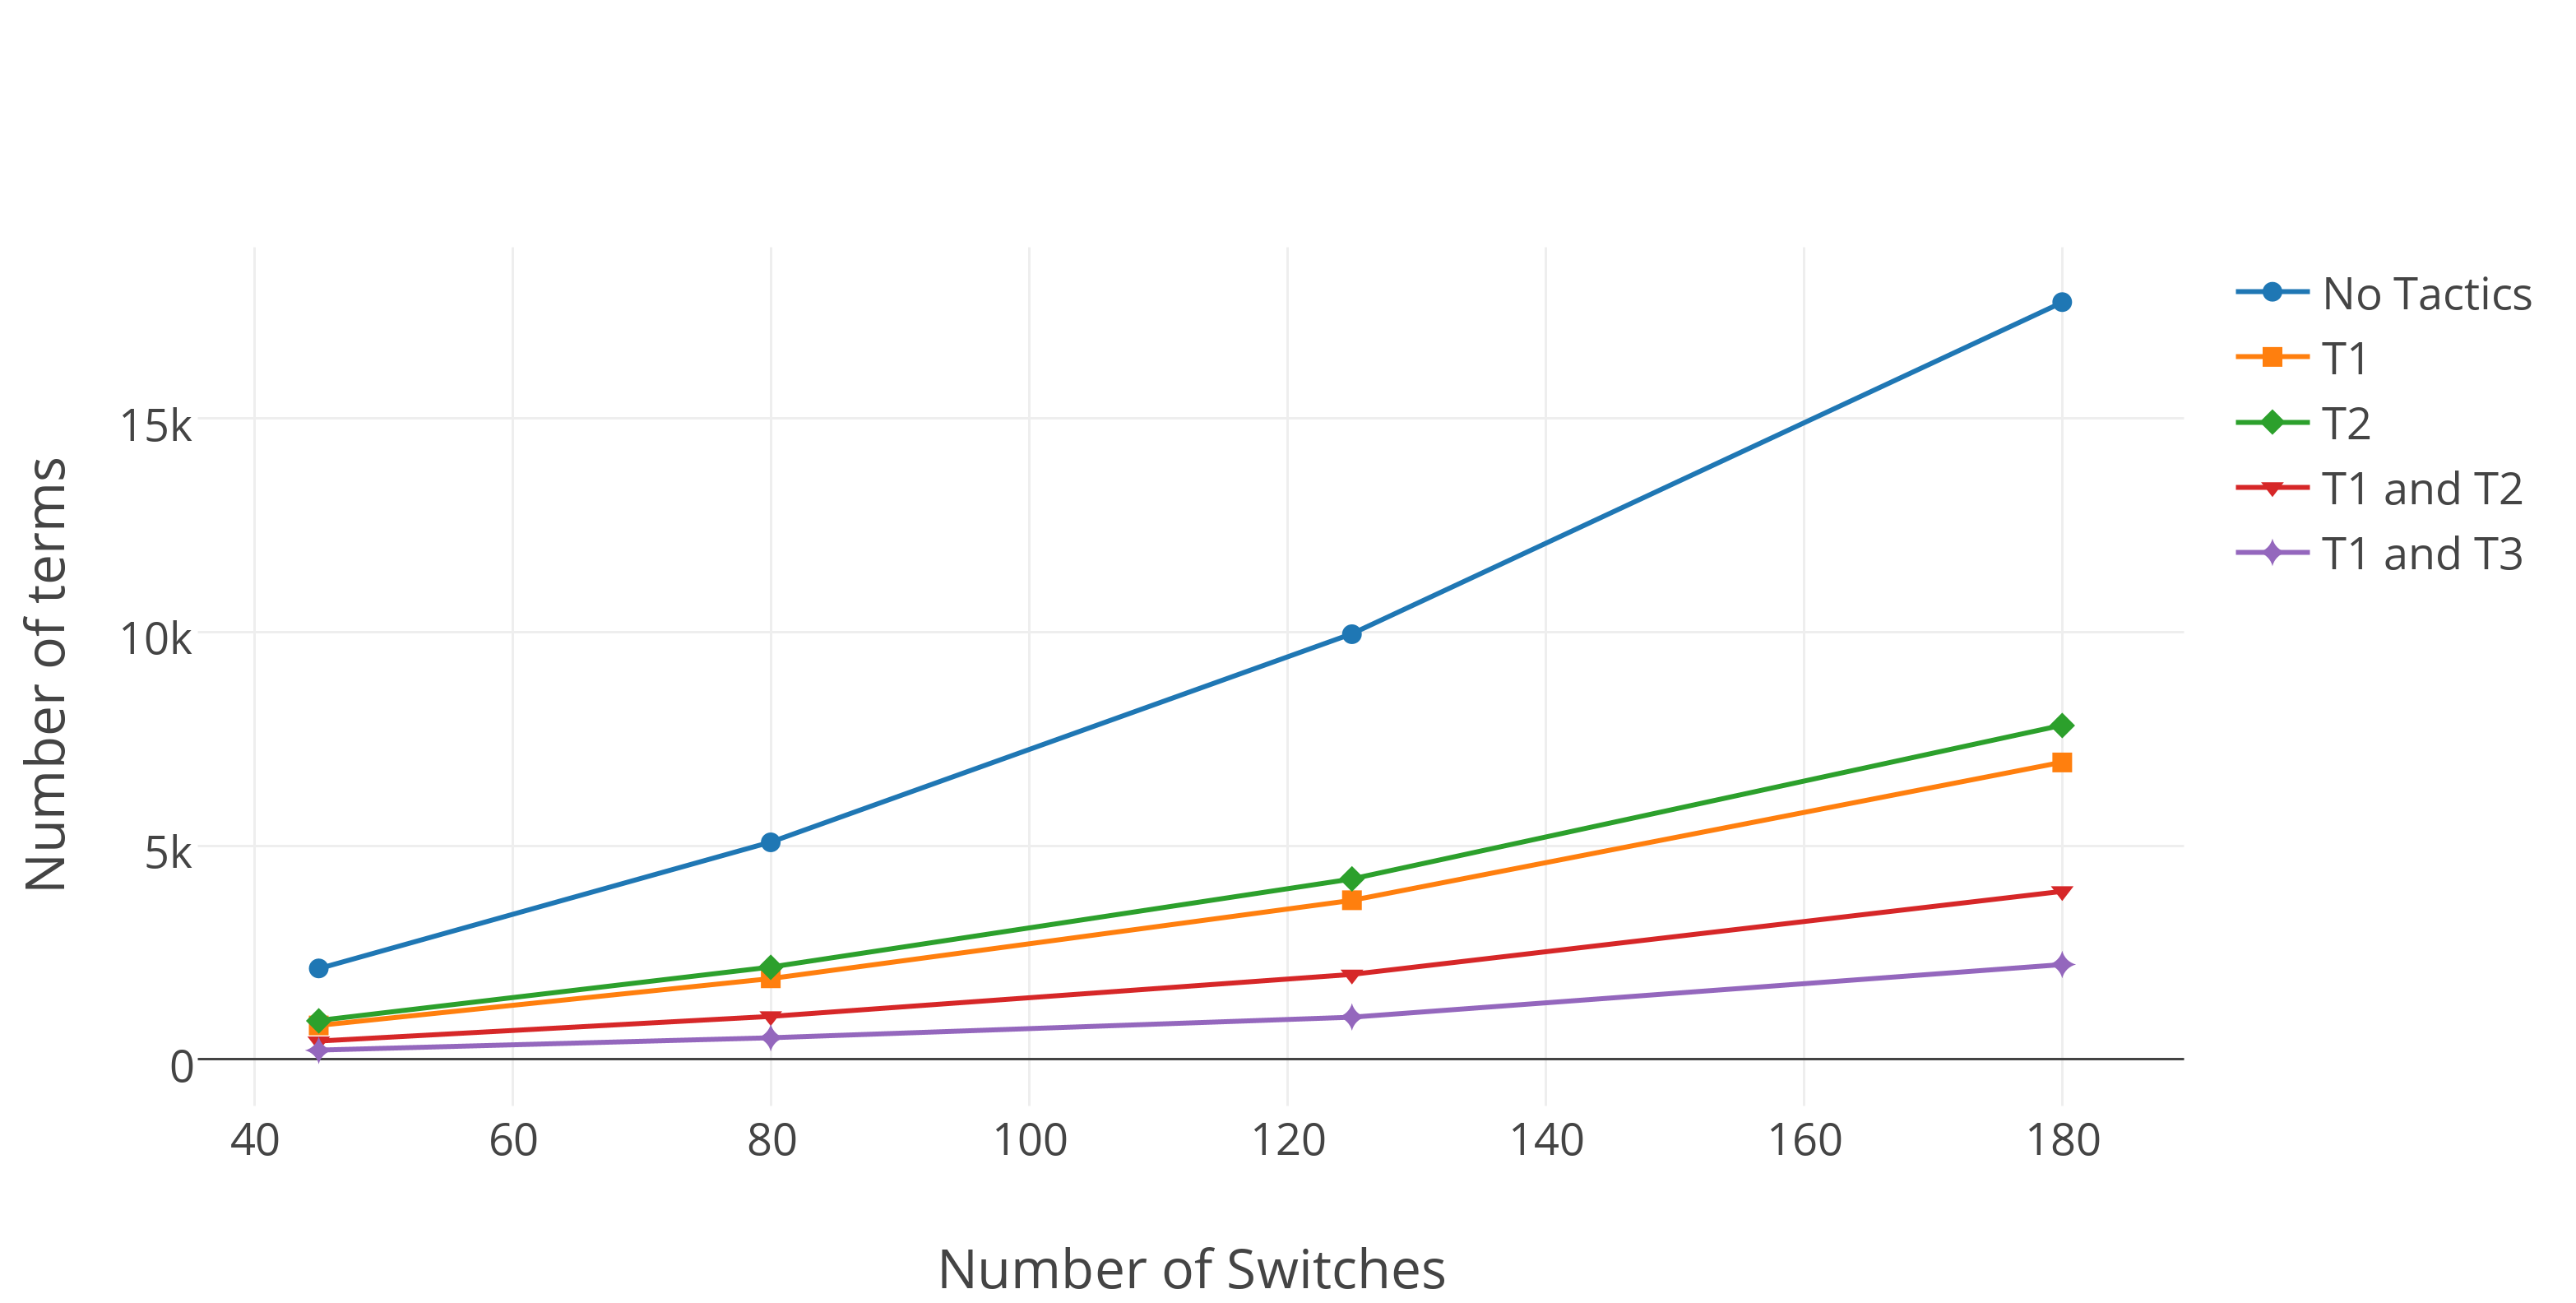
\includegraphics[height=7.5cm]{figures/tactic-reduction.png}
%	\caption{Graph used to show the reduction of terms using different tactics w.r.t the total number of terms}
%	\label{fig:tactic-reduction}
%\end{figure*}
%
%\begin{figure}
%	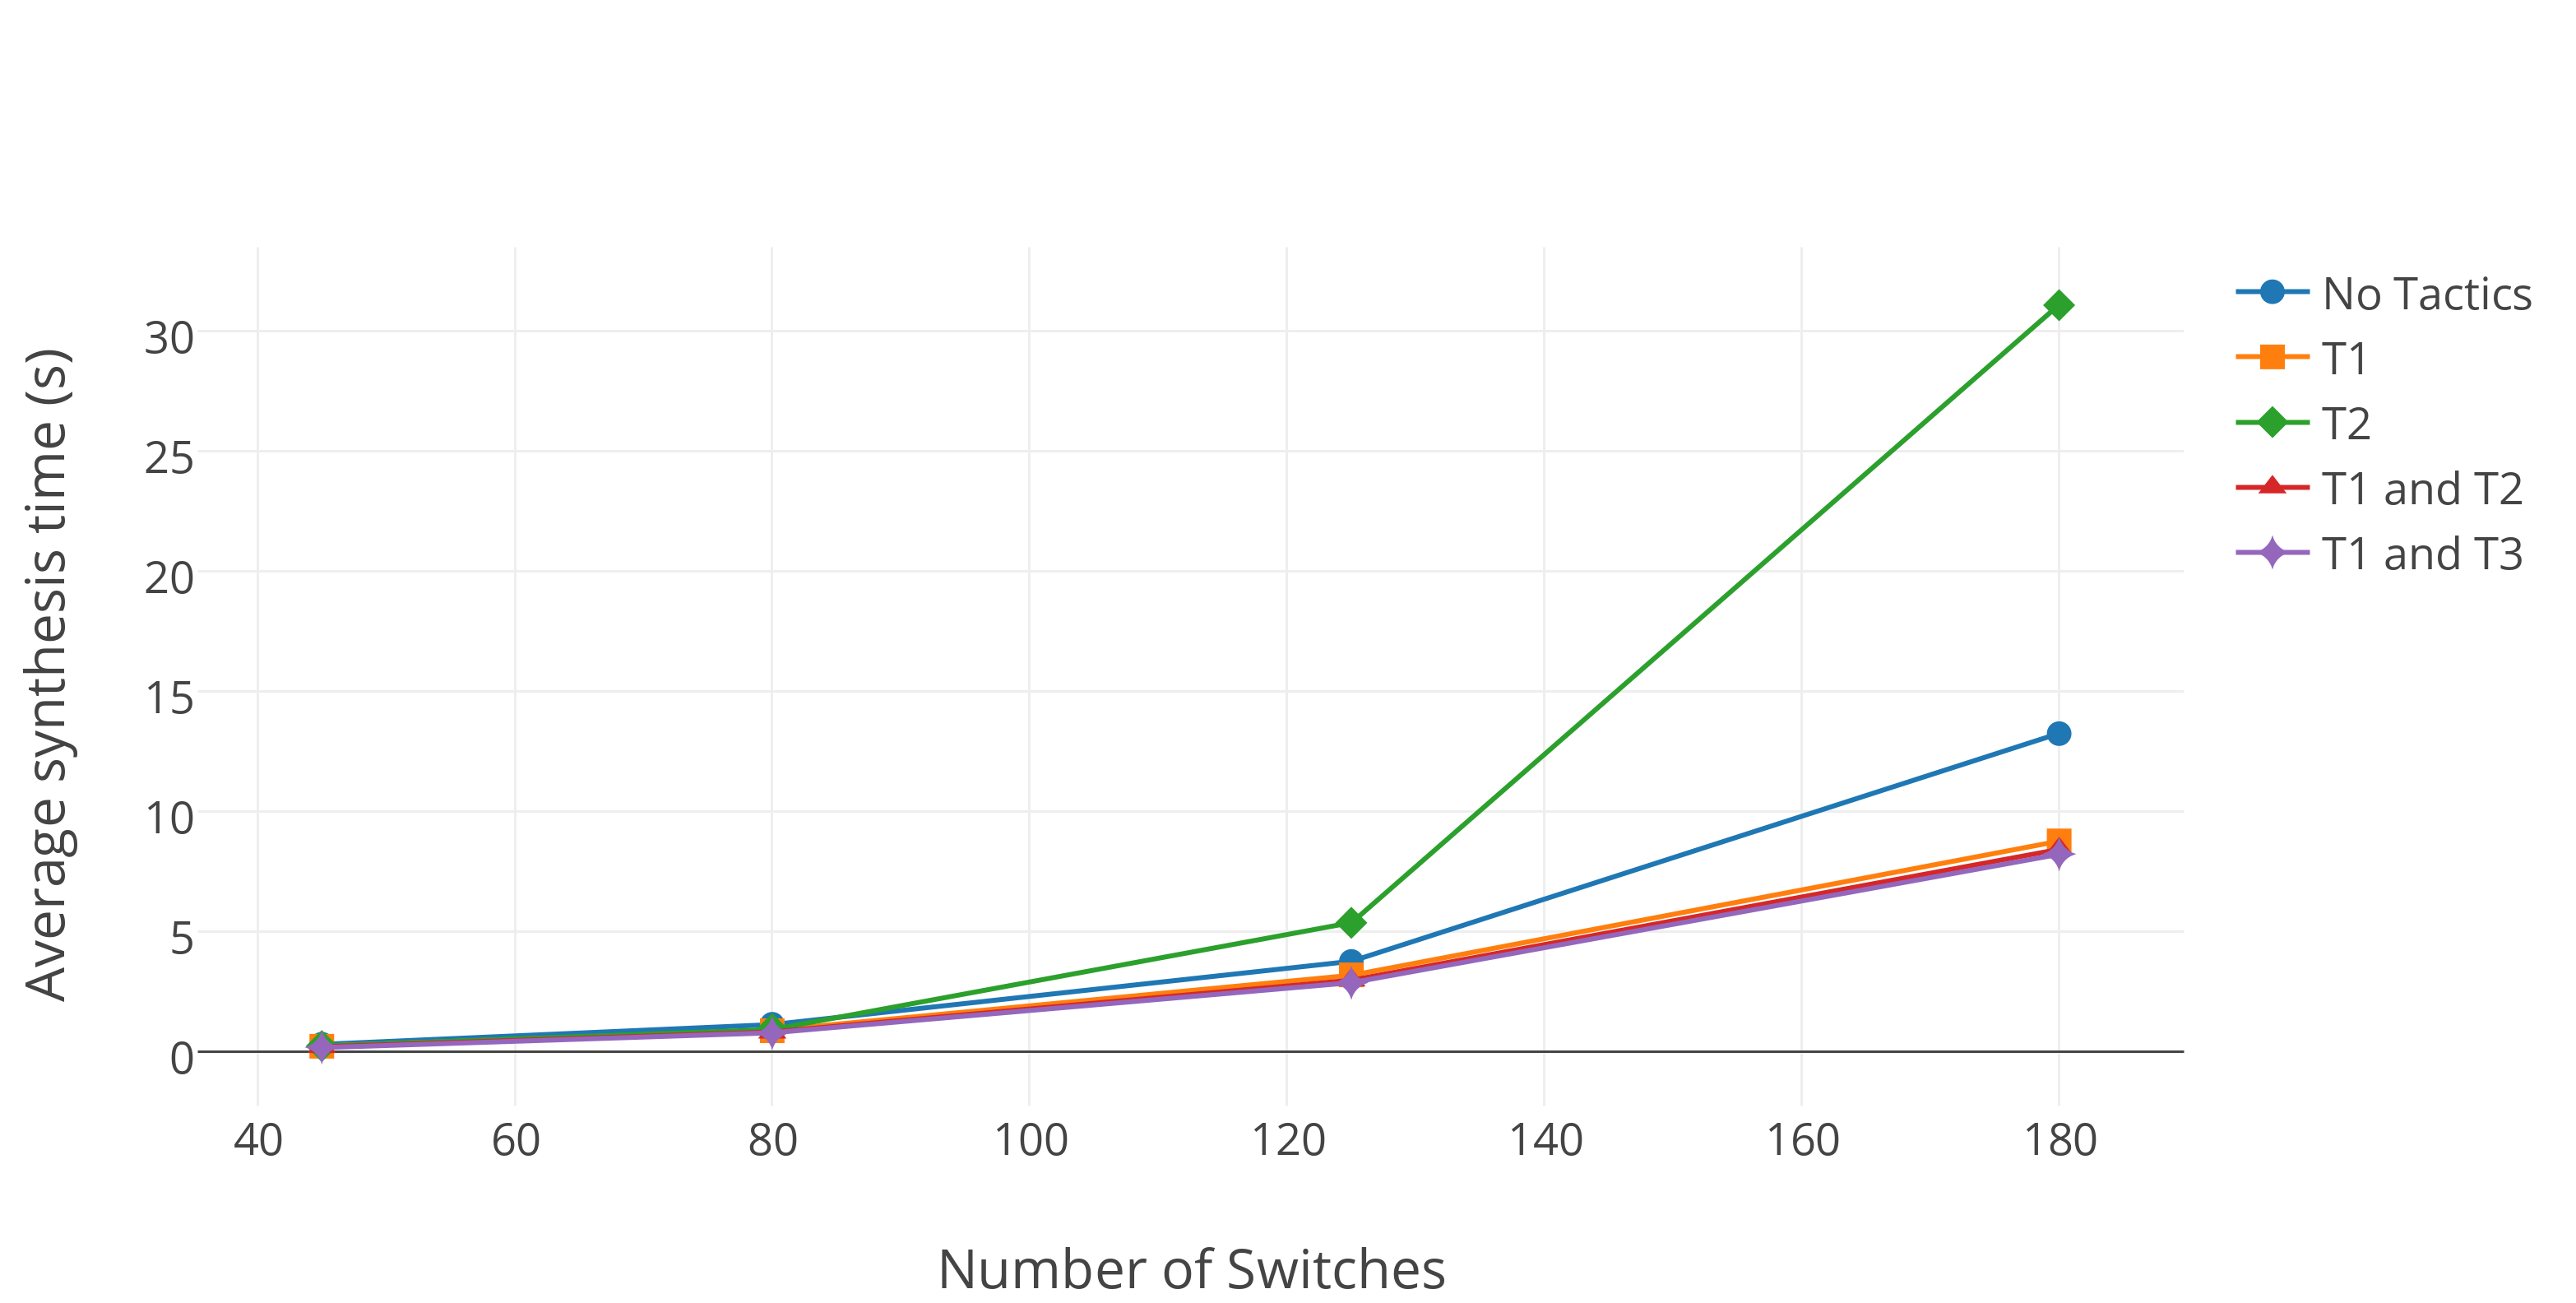
\includegraphics[width=\columnwidth]{figures/isolation-tactics.png}
%	\caption{Graph used to application of tactics for a isolation workload (percentage isolation w.r.t topology 25\%) and different topology sizes. An interesting observation in the graph is that tactics need not always help in reduction of constraints (One of the tactics, not  a very natural one) leads to more time to synthesis without tactics.}
%	\label{fig:isolation-tactics}
%\end{figure}
%
%\subsection{Optimistic Synthesis}
\begin{figure}
	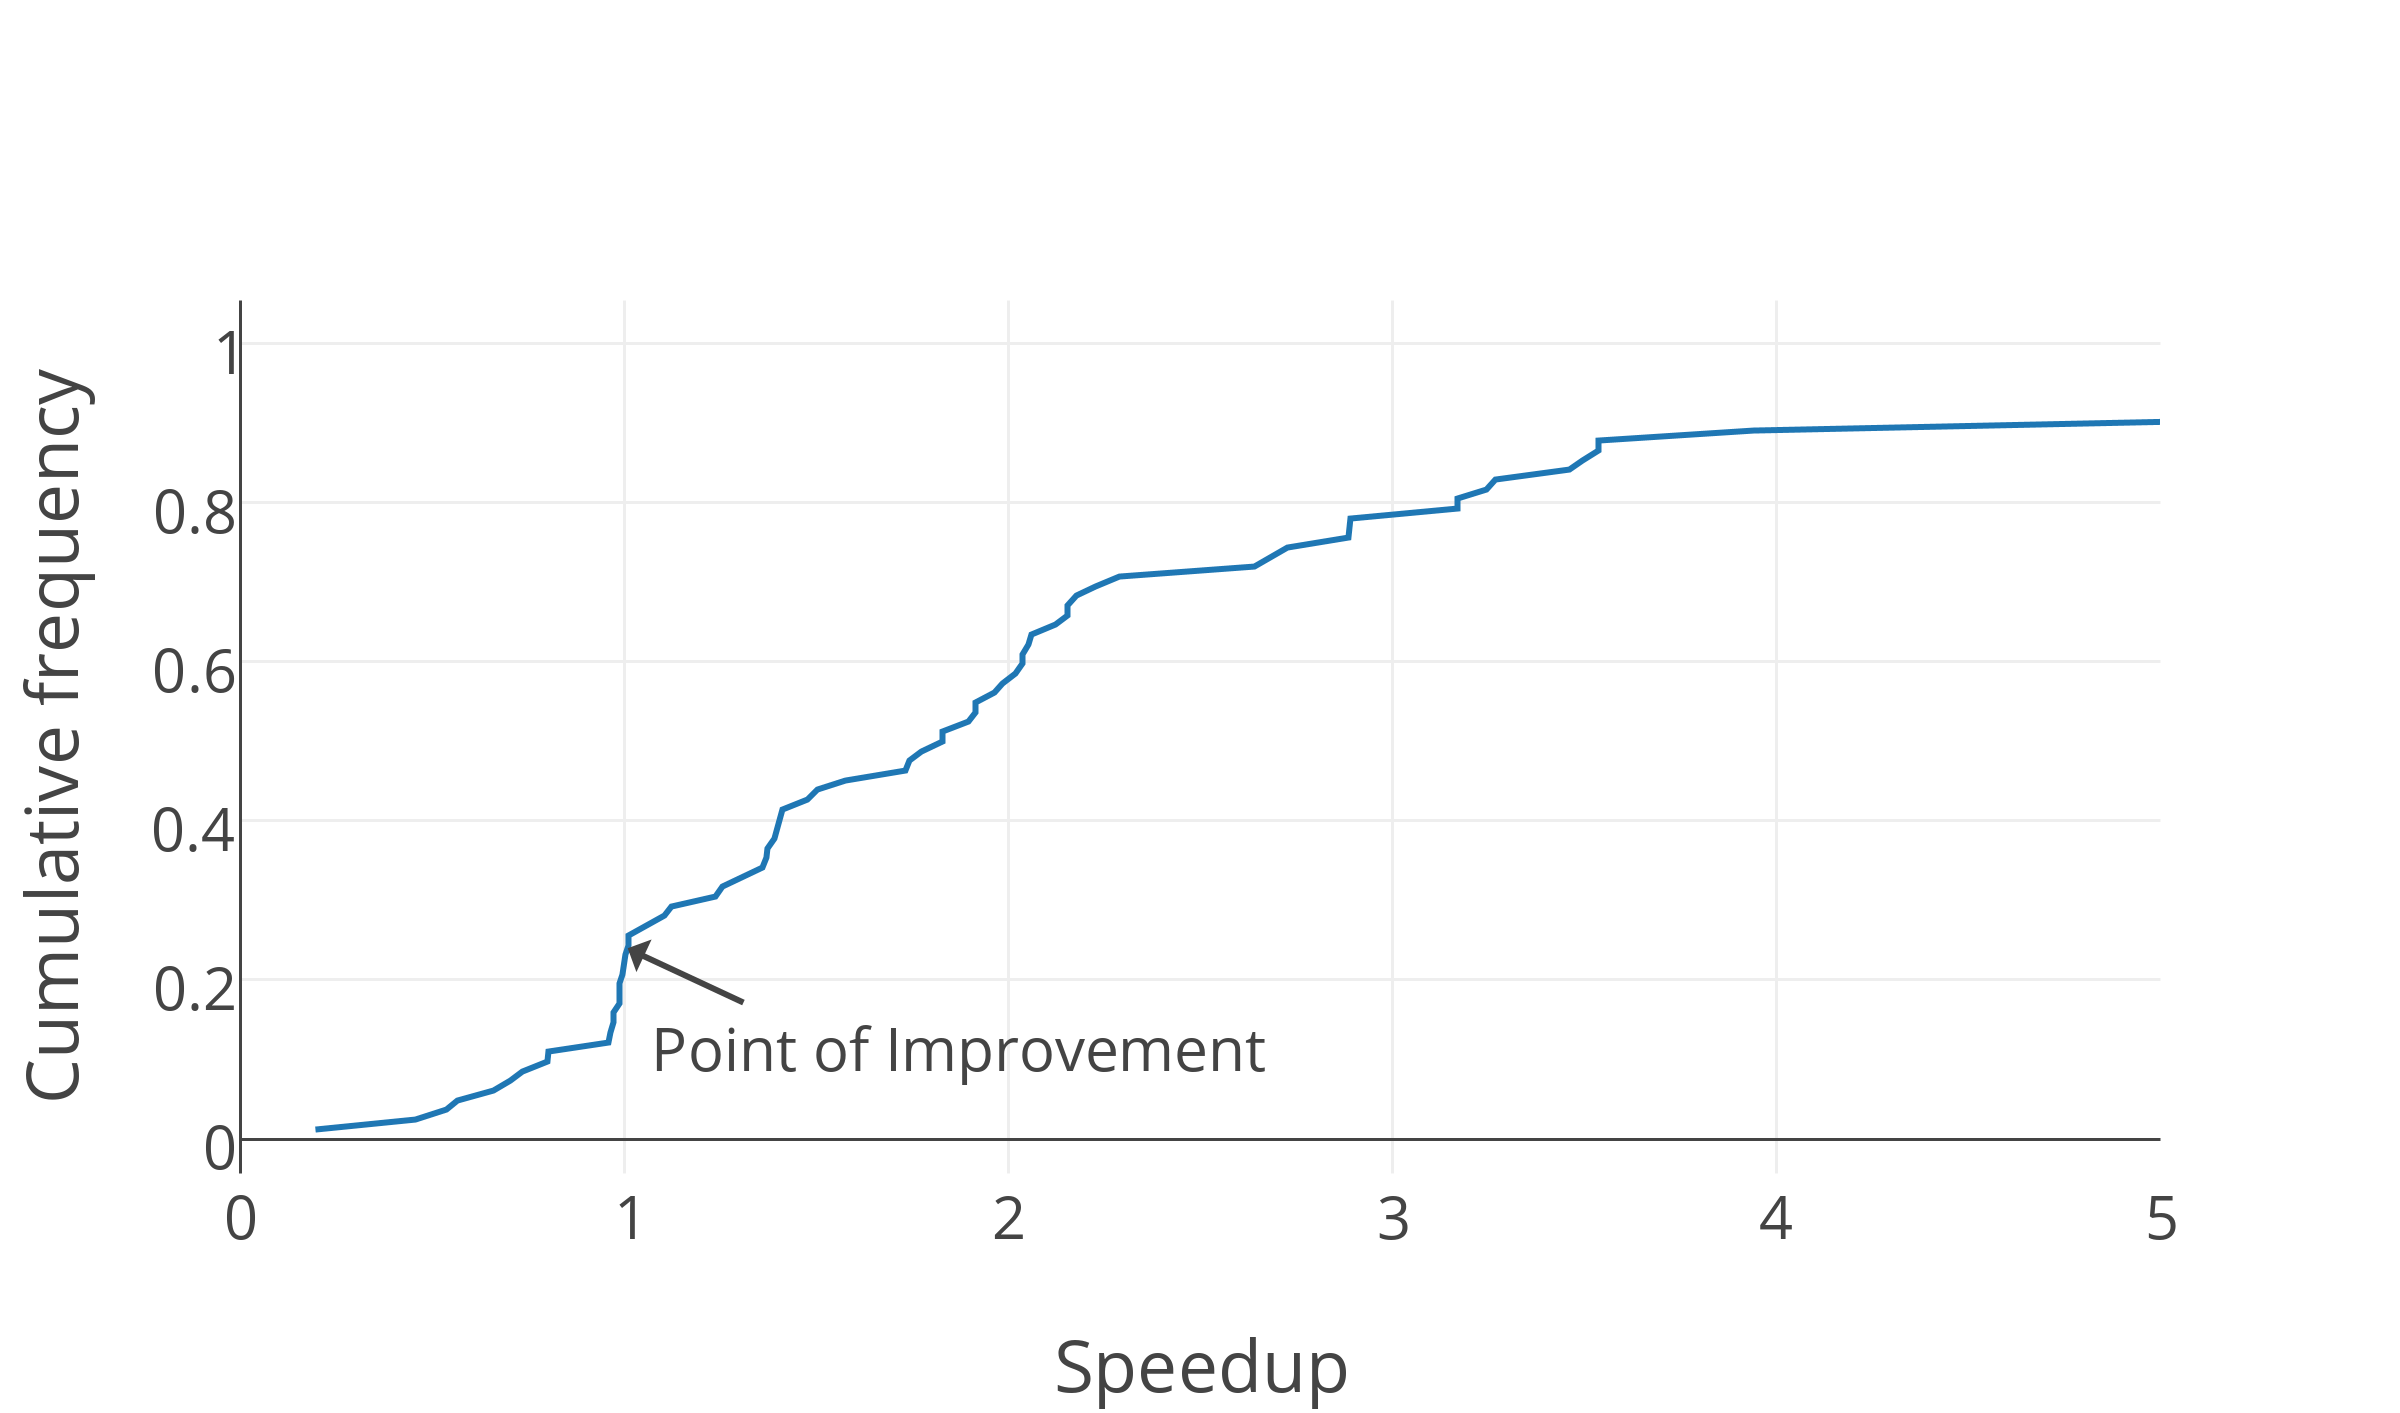
\includegraphics[width=\columnwidth]{figures/opt-cdf.png}
	\caption{Cummulative frequency distribution for speedup achieved by optimistic synthesis.}
	\label{fig:opt-cdf}
\end{figure}
\begin{figure}
	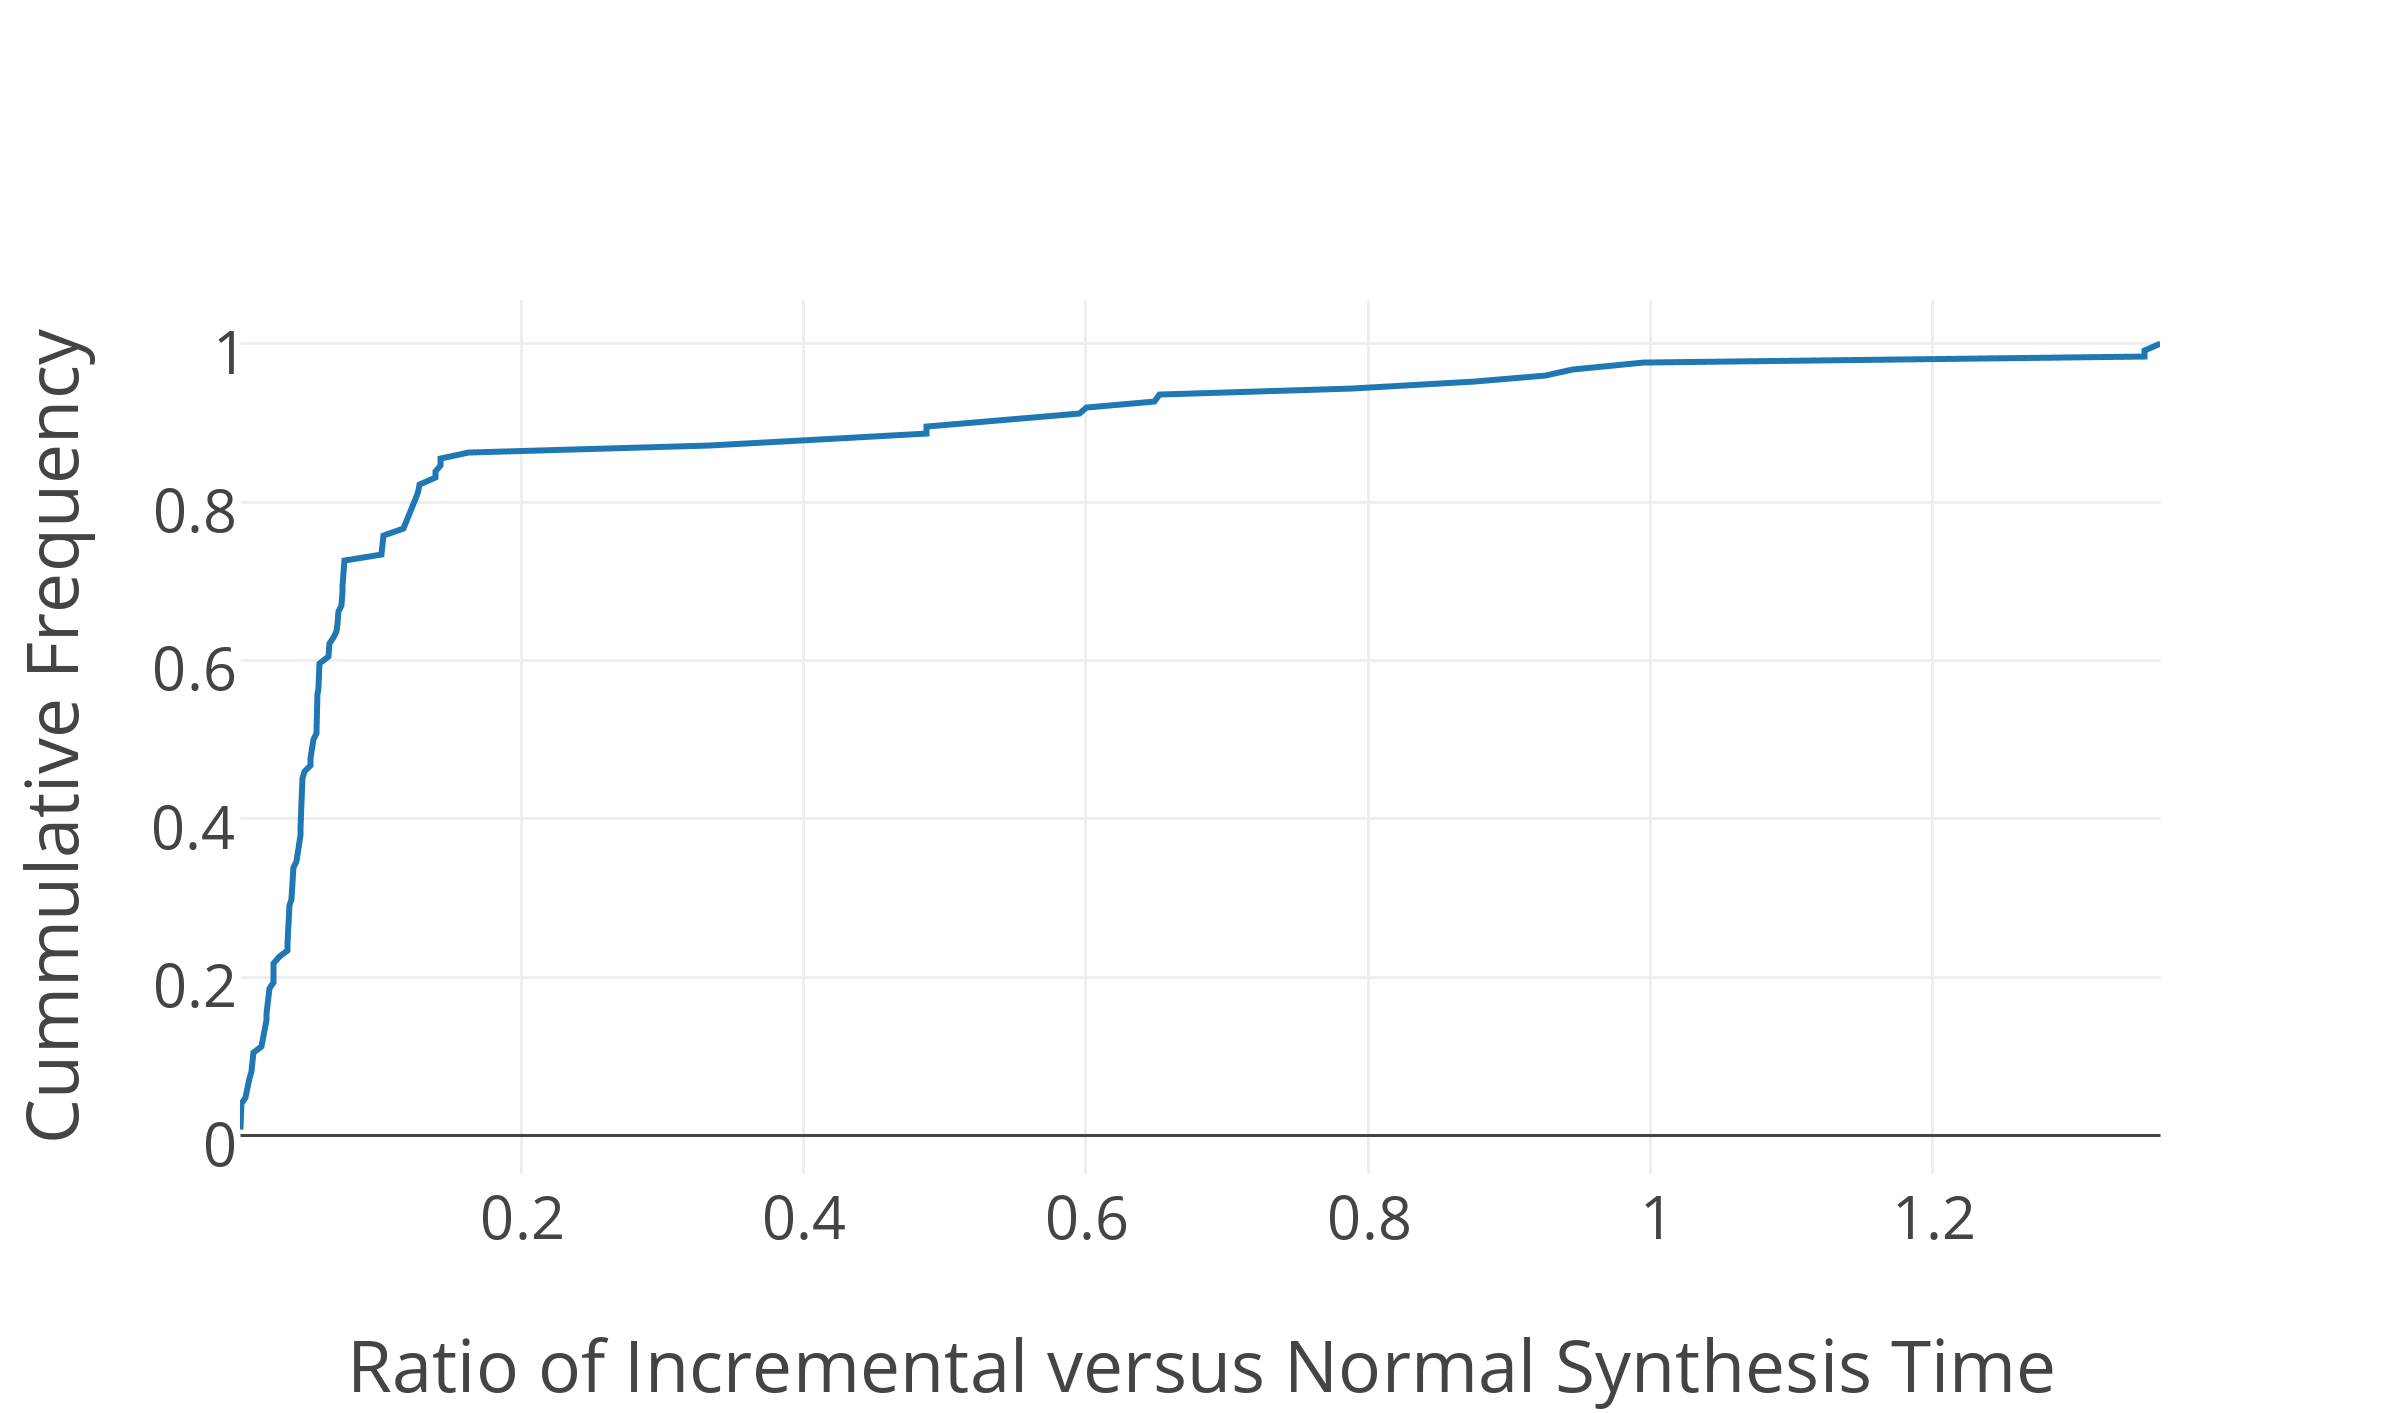
\includegraphics[width=\columnwidth]{figures/incremental-cdf.png}
	\caption{Cummulative frequency distribution for ratio of incremental synthesis/one-shot synthesis.}
	\label{fig:incremental-cdf}
\end{figure}


%\caption{Synthesis Time for varying number of reachability (with and without tactics) and waypoints policies for a 45 node fat-tree topology}


